\section{Theoretische Grundlagen}
\subsection{Entstehung von Röntgenstrahlung}
Als Röntgenstrahlen wird elektromagnetische Strahlung mit Wellenlängen zwischen 10 nm und einem Fermi bezeichnet. Um zwischen Röntgen- und $\gamma$-Strahlung unterscheiden zu können, ist die Entstehung der jeweiligen Strahlung wichtig. $\gamma$-Strahlung entsteht durch Übergänge im Atomkern während Röntgenstrahlung durch hochenergetische Übergänge in der Atomhülle oder durch Abbremsung von Elektronen entsteht. Je nach Entstehung kann die Röntgenstrahlung also ein kontinuierliches Spektrum (Bremsstrahlung) oder ein diskretes Spektrum (durch Übergänge in Atomhülle) haben.\\ \\
Um mit der Röntgenstrahlung Materialien untersuchen zu können ist es wichtig, die Entstehung des diskreten Spektrums theoretisch nachvollziehen zu können. Hierzu werden Atome mit dem Schalenmodell beschrieben. Trifft ein Elektron mit ausreichender Energie auf ein Atom kann es ein Elektron auf ein höheres Niveau anregen oder sogar Ionisieren. Damit das Atom wieder in den Grundzustand gelangt wird die entstandene Lücke durch ein Elektron aus einer höheren Schale aufgefüllt. Dieses emittiert bei dem Übergang elektromagnetische Strahlung. Wird ein Elektron aus der ersten Schale herausgelöst und durch ein Elektron aus einer höheren Schale ersetzt, spricht man bei der emittierten Strahlung von den $K$-Linie (siehe Abb. \ref{fig:k_linien}). Äquivalent sind die $L$-, $M$-,... Linien definiert, bei denen zunächst ein Elektron aus der ersten, zweiten, ... Schale herausgelöst wird. Durch die Feinstruktur werden die Linien in weitere Linien aufgespalten.
\begin{figure}[h]
  \centering
  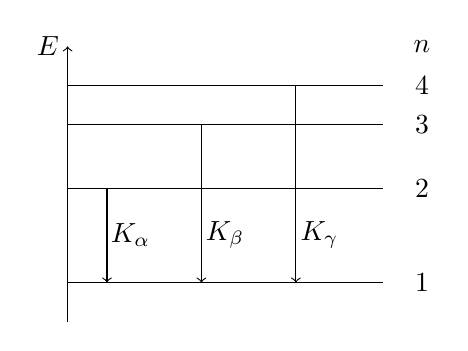
\begin{tikzpicture}
    \draw [->] (0,-3.5)--(0,0);
    \draw (-0.25,0) node {$E$};
    \draw (0,-3)--(4,-3);
    \draw (4.5,-3) node {$1$};
    \draw (0,-8*1/4+0.2)--(4,-8*1/4+0.2);
    \draw (4.5,-1.8) node {$2$};
    \draw (0,-8*1/9-0.1)--(4,-8*1/9-0.1);
    \draw (4.5,-8/9-0.1) node {$3$};
    \draw (0,-8*1/16)--(4,-8*1/16);
    \draw (4.5,-0.5) node {$4$};
    \draw (4.5,0) node {$n$};
    \draw [->](0.5,-1.8)--(0.5,-3);
    \draw (0.8,-2.4) node {$K_\alpha$};
    \draw [->](1.7,-8/9-0.1)--(1.7,-3);
    \draw (2,-2.4) node {$K_\beta$};
    \draw [->](2.9,-0.5)--(2.9,-3);
    \draw (3.2,-2.4) node {$K_\gamma$};
  \end{tikzpicture}
  \caption{$K$-Linien des charakteristischen Spektrums}
  \label{fig:k_linien}
\end{figure}

\subsection{Nachweis von Röntgenstrahlung}

Nachgewiesen werden kann die Röntgenstrahlung wegen ihrer hohen Photonenenergie durch die ionisierende Wirkung. In dem Versuch wird dabei ein Zählrohr verwendet (siehe Abb. \ref{fig:rohr}). Trifft die Röntgenstrahlung auf das Gas in dem Zylinder wird dieses ionisiert. Die freien Elektronen bewegen sich dann zur Anode und können auf dem Weg weitere Atome ionisieren. Die so verursachte Elektronenlawine erzeugt einen messbaren Strom $I$. 

\begin{figure}[h]
  \centering
  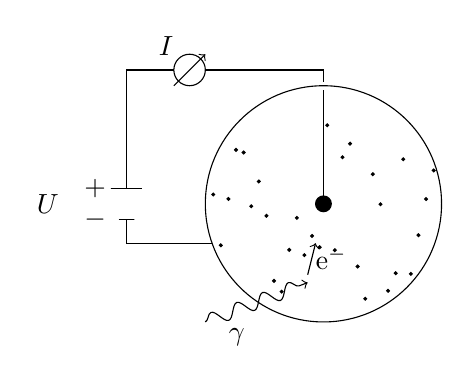
\begin{tikzpicture}
    \draw (0,0) circle (1.5);
    \draw [black, fill=black] (0,0) circle (0.1);
    \draw (0,0)--(0,1.45);
    \draw (0,1.55)--(0,1.7)--(-1.5,1.7);
    \draw (-1.7,1.7) circle (0.2);
    \draw [->] (-1.9,1.5)--(-1.5,1.9);
    \draw (-2,2) node {$I$};
    \draw (-1.9,1.7)--(-2.5,1.7)--(-2.5,0.2)--(-2.7,0.2)--(-2.3,0.2);
    \draw (-2.9,0.2) node {$+$};
    \draw (-2.9,-0.2) node {$-$};
    \draw (-3.5,0) node {$U$};
    \draw (-2.6,-0.2)--(-2.4,-0.2)--(-2.5,-0.2)--(-2.5,-0.5)--(-1.42,-0.5);
    \draw [only marks, samples=30, mark size=0.5, mark=*,domain=-1.4:1.4] plot(\x,{0.9*rand*sqrt(1.5*1.5-\x*\x)});
    \draw[decorate, decoration={snake},->] (-1.5,-1.5)--(-0.2,-1);
    \draw [->] (-0.2,-0.9)--(-0.1,-0.5);
    \draw (0.1,-0.7) node {e$^-$};
    \draw (-1.1,-1.7) node {$\gamma$};
  \end{tikzpicture}
  \caption{Querschnitt der Ionisationskammer}
  \label{fig:rohr}
\end{figure}
Die zurückbleibenden positiv geladenen Ionen bewegen sich deutlich langsamer als die Elektronen. Die positiv geladenen Atome müssen aber an der Kathode entladen werden bevor neue ELektronen ionisiert werden können. Die so vergehende Zeit, in der keine Signale erzeugt werden können, nennt sich Totzeit. \\ \\
Um die Energie der Röntgenquanten zu bestimmen wird ein Röntgenenergiedetektor verwendet. Das Funktionsprinzip beruht darauf, dass in eine PIN-Diode eindringende Röntgenquanten Elektron-Loch-Paare in der undotierten I-Zone erzeugen (Abb. \ref{fig:pin}). Dies geschieht über den Photoeffekt. Das herausgelöse Photoelektron erzeugt weitere Elektron-Loch-Paare. Durch das anliegende elektrische Feld in der Diode werden die Elektronen und die Löcher nun zu den Elektroden gezogen und somit entsteht eine messbare Spannung zwischen P- und N-Schicht. Dieses Signal wird nun verstärkt und in ein digitales Signal umgewandelt und an einen Vielkanalanalysator geleitet. Dieser zählt die Signale, sortiert in verschiedene äquidistante Energieintervalle.

\begin{figure}[h]
  \centering
  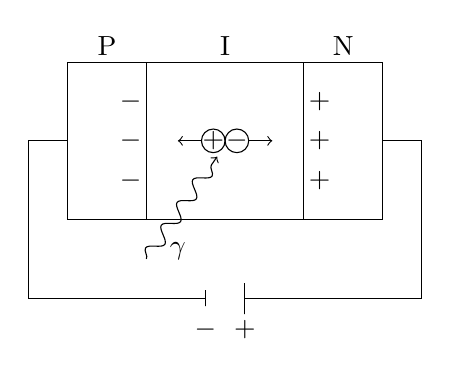
\begin{tikzpicture}
    \draw (0,0)--(0,2)--(4,2)--(4,0)--(0,0);
    \draw (1,0)--(1,2);
    \draw (3,0)--(3,2);
    \draw (0,1)--(-0.5,1)--(-0.5,-1)--(1.75,-1)--(1.75,-1.1)--(1.75,-0.9);
    \draw (4,1)--(4.5,1)--(4.5,-1)--(2.25,-1)--(2.25,-1.2)--(2.25,-0.8);
    \draw (2.25,-1.4) node {$+$};
    \draw (1.75,-1.4) node {$-$};
    \draw (0.5,2.2) node {P};
    \draw (2,2.2) node {I};
    \draw (3.5,2.2) node {N};
    \draw (0.8,1.5) node {$-$};
    \draw (0.8,1) node {$-$};
    \draw (0.8,0.5) node {$-$};
    \draw (3.2,1.5) node {$+$};
    \draw (3.2,1) node {$+$};
    \draw (3.2,0.5) node {$+$};
    \draw (1.85,1) circle (0.15);
    \draw (2.15,1) circle (0.15);
    \draw (1.85,1) node {$+$};
    \draw (2.15,1) node {$-$};
    \draw [->] (2.3,1)--(2.6,1);
    \draw [->] (1.7,1)--(1.4,1);
    \draw[decorate, decoration={snake},->] (1,-0.5)--(1.9,0.8);
    \draw (1.4,-0.4) node {$\gamma$};
  \end{tikzpicture}
  \caption{PIN-Photodiode}
  \label{fig:pin}
\end{figure}

\subsection{Zerstörungsfreie Analyse chemischer Zusammensetzungen}
Die Entstehung des charakteristischen Röntgenspektrums kann genutzt werden, um die chemische Zusammensetzung von Stoffen zerstörungsfrei zu bestimmen. Voraussetzung dafür ist, dass man die einzelnen Röntgenspektren (emittierte Energien und jeweilige Zählrate) der in der Probe enthaltenen Elemente kennt. Misst man nun das Spektrum der Probe erhält man die charakteristischen Peaks (im folgenden gekenzeichnet durch den Index) mit der jeweiligen Zählrate $H$. Nimmt man nun an, dass die Höhe der Peaks proportional zu der Zahl der Atome des jeweiligen Elements in der Probe ist folgt für den Massenanteil des $i$-ten Elements
\begin{align}
  C_i=\frac{n_iA_i}{\sum n_k A_k}=\frac{\rho_i \frac{H_i}{H_{0,i}}}{\sum \rho_k \frac{H_k}{H_{0,k}}},
\end{align}  
wobei $n_i$ die Anzahl der Atome (in der Probe), $A_i$ das Atomgewicht und $H_{0,i}$ die Zählrate im Referenzspektrum für das $i$-te Element ist. 

\subsection{Bragg-Reflexion}
Durch die Bragg-Reflexion kann die Wellenlänge von Röntgenstrahlung bestimmt werden. Der Effekt der dabei genutzt wird ist die Interferenz an einem Einkristall. Dazu wird in Abbildung \ref{fig:bragg} die Beugung von Röntgenstrahlung an zwei untereinanderliegenden Atomen des Kristalls betrachtet. Eine messbare Reflexion der Röntgenstrahlung erhält man nur dann, wenn die gebeugten Röntgenstrahlen der verschiedenen Kristallebenen konstruktiv interferieren. Mit Hilfe der Abbildung lässt sich somit die Bedingung für Konstruktive Interferenz in $n$-ter Ordnung berechnen:
\begin{align}
  2d \sin \theta=n\lambda.
  \label{eq:bragg}
\end{align} 

\begin{figure}[h]
  \centering
  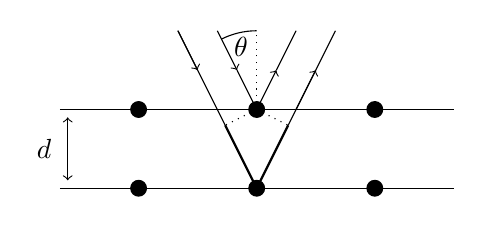
\begin{tikzpicture}
    \draw (0,1)--(5,1);
    \draw (0,0)--(5,0);
    \draw [black, fill=black] (1,0) circle (0.1);
    \draw [black, fill=black] (2.5,0) circle (0.1);
    \draw [black, fill=black] (4,0) circle (0.1);
    \draw [black, fill=black] (1,1) circle (0.1);
    \draw [black, fill=black] (2.5,1) circle (0.1);
    \draw [black, fill=black] (4,1) circle (0.1);
    \draw [<->] (0.1,0.1)--(0.1,0.9);
    \draw (-0.2,0.5) node {$d$};
    \draw [->](2,2)--(2.25,1.5);
    \draw (2.25,1.5)--(2.5,1);
    \draw [->](2.5,1)--(2.75,1.5);
    \draw (2.75,1.5)--(3,2);
    \draw [->](1.5,2)--(1.75,1.5);
    \draw [->](3,1)--(3.25,1.5);
    \draw (1.5,2)--(2.5-0.4,1-0.2);  
    \draw [thick](2.5-0.4,1-0.2)--(2.5,0)--(2.5+0.4,1-0.2);
    \draw (2.5+0.4,1-0.2)--(3.5,2);
    \draw [dotted](2.5,1)--(2.5-0.4,1-0.2);
    \draw [dotted](2.5,1)--(2.5+0.4,1-0.2);
    \draw [dotted](2.5,1)--(2.5,2);
    \draw (2.5,2) arc (90:116.6:1);
    \draw (2.3,1.8) node {$\theta$};
  \end{tikzpicture}
  \caption{Gangunterschied (fett eingezeichnet) für Bragg-Reflexion}
  \label{fig:bragg}
\end{figure}
